%Cody Lewis, Luke De Ruyter, 2012
%Visit anzhelka.com for all the latest
%
% CTRL+SPACE to switch panes in Texmaker
%
% Note: blank lines indicate a new paragraph
% Note: \left( and \right) cannot break lines.





\documentclass{article}

% Packages that are being used.
\usepackage{amsmath}
\usepackage{longtable}
\usepackage{color}
%\usepackage{verbatim} % used to display code
\usepackage{listings}
\usepackage{graphicx}

\usepackage{hyperref} %Must be at the end of use package but befor "other settings". Used to make links of all references.




\numberwithin{equation}{section} %change the numbering to have something like 1.1 and 3.15, etc.
%Format of macro:
%\newcommand{\NAME}[ARGUMENT NUMBER (OPTIONAL)]{ stuff to include, arguments denoted #1, #2, etc. }
\newcommand{\vect}[1]{\boldsymbol{#1^2}}
\newcommand{\bigvect}[3]{\boldsymbol{#1^#2^#3}}
\newcommand{\bs}[1]{\boldsymbol{#1}}

\definecolor{lightlightgray}{gray}{0.9}

\graphicspath{{../figures/}} %\graphicspath{{path/one/}{path/two/}{path/three/}}

\begin{document}



\lstset{
%language=C,                             % Code langugage
basicstyle=\ttfamily,                   % Code font, Examples: \footnotesize, \ttfamily
keywordstyle=\color{OliveGreen},        % Keywords font ('*' = uppercase)
commentstyle=\color{gray},              % Comments font
%numbers=left,                           % Line nums position
%numberstyle=\tiny,                      % Line-numbers fonts
%stepnumber=1,                           % Step between two line-numbers
%numbersep=5pt,                          % How far are line-numbers from code
backgroundcolor=\color{lightlightgray}, % Choose background color
frame=none,                             % A frame around the code
tabsize=4,                              % Default tab size
captionpos=b,                           % Caption-position = bottom
breaklines=true,                        % Automatic line breaking?
breakatwhitespace=false,                % Automatic breaks only at whitespace?
showspaces=false,                       % Dont make spaces visible
showtabs=false,                         % Dont make tabls visible
%columns=flexible,                       % Column format
%morekeywords={__global__, __device__},  % CUDA specific keywords
}








\title{Autonomous Quadrotor Project: \\ Anzhelka \\ \- \\ {\bf ALPHA DRAFT}}
\author{Cody Lewis \\ \texttt{srlm@anzhelka.com} \and Luke De Ruyter \\ \texttt{ilukester@anzhelka.com} }
\date{\today}
\maketitle
\begin{verse}\textit{
And when he [Herod] had apprehended him [Peter], he put him in prison, and delivered him to four quaternions of soldiers to keep him; intending after Easter to bring him forth to the people.} \\
\hfill --Acts 12:14, King James Bible, Cambridge Edition
\end{verse}

%% REV REV REV REV REV REV REV REV REV REV REV REV REV
\newpage
\addcontentsline{toc}{section}{Revisions}
\begin{paragraph}{Revions}
{
Here is where you will place the revisions of this document. \\ \\
9:55pm - All of the spelling was checked and fixed for the first 2 secitions writen by Luke.
5:01am - Needs to be proof read in some areas. Needs tables, conclusions, High level, references, appendices, acknowledgements
}
\end{paragraph}
%% REV REV REV REV REV REV REV REV REV REV REV REV REV

%% TOC TOC TOC TOC TOC TOC TOC TOC TOC TOC TOC TOC
\newpage
\renewcommand{\contentsname}{Table of Contents}
\tableofcontents
\addcontentsline{toc}{section}{Table of Contents}
\newpage
%% TOC TOC TOC TOC TOC TOC TOC TOC TOC TOC TOC TOC

%% S1 S1 S1 S1 S1 S1 S1 S1 S1 S1 S1 S1 S1 S1 S1 S1 S1 S1 S1 S1  

%% S1 S1 S1 S1 S1 S1 S1 S1 S1 S1 S1 S1 S1 S1 S1 S1 S1 S1 S1 S1  

%% S1 S1 S1 S1 S1 S1 S1 S1 S1 S1 S1 S1 S1 S1 S1 S1 S1 S1 S1 S1  
\section{Introduction}

A quadrotor, also known as a quadrotor helicopter or quadrocopter, is a mutlticopter that has four rotors that provide lift from a ridged frame. Quadrotor designs appeared in the 1920s, however were scraped because of bad performance and high pilot work load.

As of recent much research has gone into the developement of Unmaned Quadrotors for a wide array of uses.

In order to keep a quadrotor from spinning on its own axis, it must be built with counter rotating blades. Without counter rotating blades the quadrotor would create enough torque to spin in a constant direction around its' own axis.

Quadrotors are highly manoverable. You can take off and land vertically. You can translate horizontally through the air, you can also hold altitude. With the right pilotk(or software) behind the controls you can do amazing aerial acrobatics.

What advantages do quadrotors have over helicopters? Quadrotors have no machanical gears between the motors and propellers. Each motor is directly driving its propeller. Having four propellers allows you to have a much smaller propeller than what is on your typical heliocpopter. This means that the propellers possess less kinetic engery while spinning.
%% S1 S1 S1 S1 S1 S1 S1 S1 S1 S1 S1 S1 S1 S1 S1 S1 S1 S1 S1 S1  

%% S2 S2 S2 S2 S2 S2 S2 S2 S2 S2 S2 S2 S2 S2 S2 S2 S2 S2 S2 S2
\subsection{Executive Summary}
\begin{center}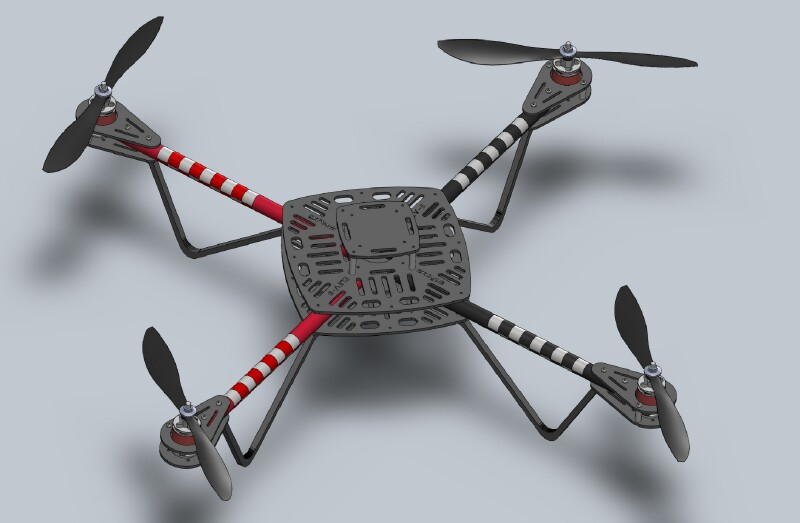
\includegraphics[scale=.6]{elev_8_rendering.JPG}\end{center}


This senior design project's goal was to create an autonomous quadrotor that would be used for outdoor sports like mountain biking, snowboarding, etc. The quadrotor would have a video camera mounted onto a gimbal that would always point at a subject/object in which the tracking device was placed. The tracking device would have its' own GPS and IMU in order to be able to determine the location and heading of the subject/object.

Our quadrotor has many features including: 3-Axis Gyro, 3-Axis Accelerometer, 3-Axis Compass, Voltage and Current monitoring of each motor, a separate battery for logic operations for emergency recoveries, ability to control up to 8 Servos, able to track the exact speed and position of each motor, monitor 8 additional analog inputs, and mounting holes for all components and future upgrades.

This senior design project was built around being Open. Open Source. Open Hardware. The frame that was used for the quadrotor was designed by Ken Gracey, an employee at Parallax, and is called the "Elev-8". There is a Git repository hosted by Google Code in which you can find all the information used and created during this senior design project. There is also a Blog which goes into some of the extensive detail that was put into this project. The main processing board for this quad rotor features a Parallax Propeller, overclocked to 100Mhz, and a fully custom board that measures in at 4 inches by 3 inches.

Testing something that is so dynamic in nature is a great challenge in its own. One of the test that has to be done in order to calculate some of the gains for the control algorithms is the motor's torque and thrust. This meant that there had to be a test stand that would test both of these constants. Another test that had to be completed was on the control board that was designed for the quadrotor.

The project was started without any expertise or experience with autonomous flying or quadrotors, but with will to learn, create and develop a system that could even be understood by people with experience in these fields. Software is one of the groups expertise. Both team members have had years of experience in multiple programming languages. Hardware on the other hand is a bit more difficult. Only Luke had any real experience with designing PCB's and circuits, however nothing to the extent of this project. The team believed that this project was worth approximately 16 credits. This was determined by the amount of hours that were being put into the project each week. Approximately 30 hours per person per week were devoted to this project.
\textcolor{red}{NEEDS ACHIEVEMENTS}
%% S2 S2 S2 S2 S2 S2 S2 S2 S2 S2 S2 S2 S2 S2 S2 S2 S2 S2 S2 S2

%% S2 S2 S2 S2 S2 S2 S2 S2 S2 S2 S2 S2 S2 S2 S2 S2 S2 S2 S2 S2  
\subsection{Design Objectives and System Overview}

This project was designed to be open ended and to be used in an unprecedented amount of ways. After watching countless videos from Go Pro cameras from a single perspectives and partial views of the subject, project Anzhelka was created. Anzhelka would allow users to be able to capture video angles that were once unattainable without costing thousands of dollars. Anzhelka would allow users to capture video with the same ease as using a Go Pro camera, but without the single perspectives and gitter from traditional methods.

The quadrotor will have at least a 15minute run time, with the abilitly to carry a 2 pound payload. It could also be controlled by a human from up to a mile away with line of sight. The control loop to keep the platform stable will run at 300Hz and be \textcolor{red}{??asynchronous??}.

On this project the team members of Anzhelka decided to keep responsibilities as open as possible, however SRLM did most of the coding and wood working while ILUKESTER did most of the embedded hardware and wiring. Everything else was either split evenly or worked on jointly.
%% S2 S2 S2 S2 S2 S2 S2 S2 S2 S2 S2 S2 S2 S2 S2 S2 S2 S2 S2 S2  

%% S2 S2 S2 S2 S2 S2 S2 S2 S2 S2 S2 S2 S2 S2 S2 S2 S2 S2 S2 S2  
\subsection{Background and Prior Art}
There have been several different renditions of this project but to the best of the teams knowledge there has not been a project that has contained the 3 main parts of this project. Autonomous Quadrotor, Object tracking, and Open.
%% S2 S2 S2 S2 S2 S2 S2 S2 S2 S2 S2 S2 S2 S2 S2 S2 S2 S2 S2 S2  

%% S2 S2 S2 S2 S2 S2 S2 S2 S2 S2 S2 S2 S2 S2 S2 S2 S2 S2 S2 S2  
\subsection{Development Environment and Tools}
%% S2 S2 S2 S2 S2 S2 S2 S2 S2 S2 S2 S2 S2 S2 S2 S2 S2 S2 S2 S2  

The Anzhelka project software was developed for the most part using a Linux system. All code and other project files are hosted on the project Git repository (code.anzhelka.com). The Propeller code was written in Gedit, compiled and downloaded with the BSTC compiler, and interfaced with using picocom.

%% S3 S3 S3 S3 S3 S3 S3 S3 S3 S3 S3 S3 S3 S3 S3 S3 S3 S3 S3 S3  
\subsubsection{Directory Structure}
%% S3 S3 S3 S3 S3 S3 S3 S3 S3 S3 S3 S3 S3 S3 S3 S3 S3 S3 S3 S3  

The project uses the following directory structure:
\begin{lstlisting}
 /hardware 
    /frame 
    /pcb 
 /software 
    /spin 
       /src 
       /lib 
       /test 
       /tool 
       /config 
    /java 
       /src 
       /lib 
       /test 
       /tool 
       /config 
 /doc 
    /datasheet 
    /reports 
    /figures 
    /notes 
    /tests 
    /extra 
 /extra 
\end{lstlisting} 
 
 
\texttt{Hardware}
Subfolders will store the major components of the project. For example, the frame has several .dxf files that are sent to the laser cutter, so that will all go into a subfolder called frame. The project may have several PCBs made as well, and so each should go into a subfolder under pcb. 

\texttt{Software}
The software is separated by language into separate folders. This makes sense because each processor in the project will have only one language running, but separate processors that are running the same language may share components (library files, for example). Each language has a number of subfolders: 

\begin{list}{*}{}
	\item src is where the source code for the project is stored. Subfolders as appropriate. 
	\item lib stores all general purpose library files (code) such as Propeller Obex objects. 
	\item test stores the test harnesses such as unit tests and Spin code to test a particular module (the latter case would have a 'main' type method and would be self supporting when running on the Propeller). 
	\item tool holds all the relevant development tools for that language (bstc for Spin, for example). 
	\item config stores any sort of relevant compile time or testing configuration files. 
\end{list}
The files that are in the Software folder should be used only for what runs onboard the quadrotor. Test programs or desktop PC client programs should instead go into the Extra folder. Note that these programs may still access the lib and tool subfolders in the software directory. 

\texttt{Documentation}
This folder stores all the relevant datasheets in the datasheet subdirectory, and any other project documentation that is deemed to fit. Note that most documentation probably belongs in the anzhelka wiki. 

The datasheet and reports folder contain the reference datasheets for each component and the various generated reports of the project, respectively. The figures folder holds an images that is used in the documentation. The notes folders holds papers that are interesting and relevant to the project, such as the cited research papers. The tests folder holds the test results data, and any associated data processing scripts. The extra folder holds other documentation material such as project logos and fonts. 

\texttt{Extra}
This folder contains other associated programs for the project. Since the Software folder is dedicated exclusively to software that is intended to fly the quadrotor other programs need to be stored in the Extra folder. This folder stores the Anzhelka Terminal files and the Thrust/Torque test stand files for example.

All code is compiled with the BSTC compiler. This is available in \cite{campbell09}. This compiler was selected because it is Linux compatible and it has several optimizations over the Parallax provided compiler. In addition, it has a command line interface which makes it easy to integrate into a compilation cycle script. BSTC will also download the compiled code via the USB COM port to the Propeller.

%% S3 S3 S3 S3 S3 S3 S3 S3 S3 S3 S3 S3 S3 S3 S3 S3 S3 S3 S3 S3  
\subsubsection{Development Cycle}
%% S3 S3 S3 S3 S3 S3 S3 S3 S3 S3 S3 S3 S3 S3 S3 S3 S3 S3 S3 S3  
To facilitate the development cycle a simple compilation script was developed. A template form of this script can be found in $/software/spin/tool/bst_template.sh$. This script will compile the Spin program, and if no errors are found it will attempt to download to the Propeller. If successful it will open picocom (terminal program) on the USB port to listen for data. Using this script while programming dramatically decreases the write-compile-test debug cycle.

All code was written in Gedit. Gedit is a simple text editor with a few features built in, including syntax highlighting. For most of the languages in this project, Gedit has provided suitable syntax highlighting. Propeller Spin, however, is not available by default. Syntax highlighting was accomplished by writing a language definition file ($/software/spin/tool/spin.lang$) and placing it in $/usr/share/gtksourceview-3.0/language-specs$. Gedit will then automatically highlight the Spin files.

%%TODO: update the file path typesetting.

All project files are hosted on the project Git repository, hosted by Google Code at code.anzhelka.com. A Git repository was selected so that all developers would have equal access to the source files, changes would be logged and trackable, issues would be trackable, and so that concurrent work on files  could be easily merged. All project files are open source under the MIT license and can be downloaded freely.

%% S2 S2 S2 S2 S2 S2 S2 S2 S2 S2 S2 S2 S2 S2 S2 S2 S2 S2 S2 S2  
\subsection{Definitions and Acronyms}
\textcolor{red}{Needs lots more of definitions}\\
\begin{tabular}{l l}
	BSTC & Brad's Spin Tool Compiler \\
	ESC & Electronics Speed Control \\
	IMU & Inertial Messurement Unit \\
	PWM & Pulse Width Modulation \\
	PCB & Printed Circuit Board \\
	RISC & Reduced Instruction Set Computing\\
	PASM & Propeller Assembly \\
	RAM & Random Access Memroy \\
	GUI & Graphical User Interface \\
	AT & Anzhelka Terminal \\
	\$ADxxx & Anzhelka Terminal Data Type \\
	OOP & Object Orianted Programming \\
	EEPROM & Electrically Erasable Programmable Read-Only Memory \\
	PID & Proportional-Integral-Derviavtive \\
	UART & Universal Asynchronous Receiver /Transmitter (serial) \\
\end{tabular}
%% S2 S2 S2 S2 S2 S2 S2 S2 S2 S2 S2 S2 S2 S2 S2 S2 S2 S2 S2 S2



%% S1 S1 S1 S1 S1 S1 S1 S1 S1 S1 S1 S1 S1 S1 S1 S1 S1 S1 S1 S1  
\section{Requirements Specifications}
\textcolor{red}{This section describes issues that need to be addressed or resolved prior or while completing the design as well as issues that may influence the design process. \\ \\ Still needed?}
%% S1 S1 S1 S1 S1 S1 S1 S1 S1 S1 S1 S1 S1 S1 S1 S1 S1 S1 S1 S1  


%% S2 S2 S2 S2 S2 S2 S2 S2 S2 S2 S2 S2 S2 S2 S2 S2 S2 S2 S2 S2  
\subsection{Assumptions}
Have you ever mounted a camera on to your helmet and rode down a mountainous trail? What about trying to capture yourself while water skiing? Watching the video usually turns out shaky and in one perspective. Would it be nice to be able to see what you did wrong that caused you to fall of your bike? Most of the time you can't see what went wrong. What if you could do all of that while still capturing amazing views?  All this can be accomplished while being as simple as powering on a couple of devices. 
%% S2 S2 S2 S2 S2 S2 S2 S2 S2 S2 S2 S2 S2 S2 S2 S2 S2 S2 S2 S2  


%% S2 S2 S2 S2 S2 S2 S2 S2 S2 S2 S2 S2 S2 S2 S2 S2 S2 S2 S2 S2  
\subsection{Realistic Constraints}
Every system has constraints and Anzhelka is no exception. Our quadrotor can only travel so fast, about 10 mph, therefore it wouldn't be able to keep up with anything much faster than that. Large gust of wind could cause problems with keeping the quadrotor platform stable enough to keep the camera from shaking. Wet weather would be large problem and would cause unknown and uncalculated problems.

%% S2 S2 S2 S2 S2 S2 S2 S2 S2 S2 S2 S2 S2 S2 S2 S2 S2 S2 S2 S2  

%% S2 S2 S2 S2 S2 S2 S2 S2 S2 S2 S2 S2 S2 S2 S2 S2 S2 S2 S2 S2  
\subsection{System Environment and External Interfaces}

To be able to accomplish all of these tasks there are many of interfacing between many different devices. Our main control board must control all 4 ESC's, communicate with the IMU via a serial UART, servos must be controlled via PWM signals, voltage and current of each motor is monitored via a specially designed circuit.
%% S2 S2 S2 S2 S2 S2 S2 S2 S2 S2 S2 S2 S2 S2 S2 S2 S2 S2 S2 S2   

%% S2 S2 S2 S2 S2 S2 S2 S2 S2 S2 S2 S2 S2 S2 S2 S2 S2 S2 S2 S2  
\subsection{Budget and Cost Analysis}
Unfortunately there was no money that was given to the team in order to support the project. All of the funding had come from the team members own personal accounts. Below is an exert from our spreadsheet with the cost analysis and money spent on this project.
\textcolor{red}{INSERT COST TABLE HERE}\\ \\
\textcolor{blue}{Update table before adding}
%% S2 S2 S2 S2 S2 S2 S2 S2 S2 S2 S2 S2 S2 S2 S2 S2 S2 S2 S2 S2

%% S2 S2 S2 S2 S2 S2 S2 S2 S2 S2 S2 S2 S2 S2 S2 S2 S2 S2 S2 S2  
\subsection{Safety}

When dealing with any autonomous system one must take extreme cautions in order to insure the safety of everyone. Autonomous systems are dangerous because there is no one behind the controls of the system and can become unpredictable in the event of a system failure. 

During the design process of the frame the team made sure to use fasteners, washers, and nuts that were of suitable specification. In addition, all threaded components were secured using blue lock tight to ensure that nothing would loosen on its own.

Whenever flying an aerial vehicle be sure to wear safety glasses to protect your eyes in the event that the propeller has a failure and is detached/released from the motor(s).
%% S2 S2 S2 S2 S2 S2 S2 S2 S2 S2 S2 S2 S2 S2 S2 S2 S2 S2 S2 S2  

%% S2 S2 S2 S2 S2 S2 S2 S2 S2 S2 S2 S2 S2 S2 S2 S2 S2 S2 S2 S2  
\subsection{Importance of Team Work}
Being able to work in a team is both a skill and a challenge. Working on a project in a group helps you split up the work load and possibly get more work done in less time, however being able to work together with others on the project could present a greater challenge than the project itself. 

This was a foreseen challenge and the team set up a Git repository for all code, data, images, and presentations. There was also an official blog set up where we could go in great detail on what we were working on and we had yet to complete. With these two resources set up and with the help of keeping an open schedule the team has come to realize how important team work really is.
\\ \\
\textcolor{red}{Cody's Input}
%% S2 S2 S2 S2 S2 S2 S2 S2 S2 S2 S2 S2 S2 S2 S2 S2 S2 S2 S2 S2

%% S1 S1 S1 S1 S1 S1 S1 S1 S1 S1 S1 S1 S1 S1 S1 S1 S1 S1 S1 S1  
\section{System Design}
\textcolor{green}{\bf System Design—this level of design includes the entire system, including the people and processes involved, and not just the software architecture.}
\textcolor{red}{Cody}
%% S1 S1 S1 S1 S1 S1 S1 S1 S1 S1 S1 S1 S1 S1 S1 S1 S1 S1 S1 S1

%% S2 S2 S2 S2 S2 S2 S2 S2 S2 S2 S2 S2 S2 S2 S2 S2 S2 S2 S2 S2  
\subsection{Experiment Design}
%% S2 S2 S2 S2 S2 S2 S2 S2 S2 S2 S2 S2 S2 S2 S2 S2 S2 S2 S2 S2  

%% S2 S2 S2 S2 S2 S2 S2 S2 S2 S2 S2 S2 S2 S2 S2 S2 S2 S2 S2 S2  
\subsection{Experiment Results and Feasibility}
%% S2 S2 S2 S2 S2 S2 S2 S2 S2 S2 S2 S2 S2 S2 S2 S2 S2 S2 S2 S2  

%% S1 S1 S1 S1 S1 S1 S1 S1 S1 S1 S1 S1 S1 S1 S1 S1 S1 S1 S1 S1  
\section{Software Introduction}

%% S2 S2 S2 S2 S2 S2 S2 S2 S2 S2 S2 S2 S2 S2 S2 S2 S2 S2 S2 S2  
\subsection{Propeller}

%% S3 S3 S3 S3 S3 S3 S3 S3 S3 S3 S3 S3 S3 S3 S3 S3 S3 S3 S3 S3  
\subsubsection{Architecture}

The Anzhelka project uses the Propeller P8X32A microcontroller from Parallax. This microcontroller is a 8 core 32 bit RISC processor. The Propeller is \$8 per chip, plus approximately \$2 for support components. For this project the Propeller has been overclocked from the default 80MHz to 100MHz. This additional speed facilitates more complex computations without sacrificing output rate. Each core, called a COG, is identical with equal access to all chip resources. The Propeller has a central RAM area called the HUB which is COG accessible in a round robin fashion.

The Propeller is distinctly different from most other microcontrollers by it's lack of built in hardware. The Propeller does not have any hardware level serial ports, analog to digital or digital to analog ports, or any pulse width modulation ports. Instead, the Propeller is designed to be able to use software for these common interfaces. This is typically done through what is known as “bit banging.” The only exception is the built in video generation hardware that assists in creating NSTC, PAL, or VGA signals. To make development easier for the programmer, Parallax hosts a source code website that provides code for common tasks such as serial or PWM.

The Propeller has two built in languages: a high level language called Spin and the assembly language called PASM. PASM is executed directly by a COG. Spin is executed by a built in PASM Spin interpreter that can be dynamically loaded into one or more COGs. Other high level languages available for the Propeller generally operate in a similar manner to Spin. This project uses Spin and PASM exclusively.

The Propeller has three different memory locations: 2KB of COG RAM, 32KB of HUB RAM, and external 64KB of I2C EEPROM. Upon startup, the Propeller copies the contents of the EEPROM to HUB RAM, loads a Spin interpreter into COG 0, and begins execution.  Any PASM code, including the Spin interpreter, must fit in 496 instructions or less in order to fit into the COG RAM. The Propeller does not have provisions for fetching PASM instructions from other locations besides COG RAM. For Spin code the compiled interpretable bytes are stored in the HUB RAM, and are fetched and decoded by the Spin interpreter.
%% S3 S3 S3 S3 S3 S3 S3 S3 S3 S3 S3 S3 S3 S3 S3 S3 S3 S3 S3 S3  

%% S3 S3 S3 S3 S3 S3 S3 S3 S3 S3 S3 S3 S3 S3 S3 S3 S3 S3 S3 S3  
\subsubsection{Programming}

The Propeller is programmed in PASM and a high level language called Spin. In general, PASM is used when speed is required. At 100MHz, the Propeller can execute 25,000,000 assembly instructions each second (each instruction takes 40ns). By contrast, the interpreted Spin language is about 100x slower. Because of this contrast Spin is used where ease of programming is important, and PASM is used where speed is important.

Spin is officially called an object oriented programming language, but there are some subtle differences compared to mainstream object oriented terminology. Spin OOP is used to organize code into logical blocks much like an import statement in C++ or Python. Spin objects do not use techniques such as class instances, inheritance, subtype polymorphism. A Spin object is used to group related functions together into a unit that can be included in multiple Spin programs. Typically, Spin objects are used for interfacing with external devices. For example, a typical Spin program might have an object for serial communication, an object for VGA signal generation, and an object for I2C communication. The Parallax Object Exchange ([REFERENCE]) hosts Parallax written objects and community written objects under the open source MIT licence.

Spin syntax is very similar to Python. To denote a new scope Spin uses indentation instead of curly braces {} (familiar to C/C++ and Java programmers). Spin code is divided into blocks: CON (constant), VAR (variable), OBJ (object), DAT (data), PUB (public function), and PRI (private function). Most typical programming constructs are a part of the Spin language: conditional IF statements, FOR loops (called REPEAT), boolean conditions, and so on.

All variables in the Propeller are integers. Variables are typically 32 bit signed integers called longs, but in Spin it is possible to create 16 bit or 8 bit sized variables as well (called words and bytes, respectively). Global variables are declared in the VAR block, and global constants are declared in the CON block. PRI and PUB functions can declare local variables, along with function parameters. 
%% S3 S3 S3 S3 S3 S3 S3 S3 S3 S3 S3 S3 S3 S3 S3 S3 S3 S3 S3 S3  
%% S2 S2 S2 S2 S2 S2 S2 S2 S2 S2 S2 S2 S2 S2 S2 S2 S2 S2 S2 S2  


%% S2 S2 S2 S2 S2 S2 S2 S2 S2 S2 S2 S2 S2 S2 S2 S2 S2 S2 S2 S2  
\subsection{Other Software Stuff}
\textcolor{red}{Cody...} ie things such as the python and the possibility of future expansion (BeagleBoard)


%% S2 S2 S2 S2 S2 S2 S2 S2 S2 S2 S2 S2 S2 S2 S2 S2 S2 S2 S2 S2  

%% S1 S1 S1 S1 S1 S1 S1 S1 S1 S1 S1 S1 S1 S1 S1 S1 S1 S1 S1 S1  
  

%% S1 S1 S1 S1 S1 S1 S1 S1 S1 S1 S1 S1 S1 S1 S1 S1 S1 S1 S1 S1  
\section{Quadrotor Prototype Construction}
%\textcolor{green}{\bf Given the relatively short duration of the class, completion of the project may not be possible; however, you must do your best to produce a working prototype that implements the most important core functionality of the system you have envisions. If graphical output is not possible, create some screen mock-ups on your own.}
%% S1 S1 S1 S1 S1 S1 S1 S1 S1 S1 S1 S1 S1 S1 S1 S1 S1 S1 S1 S1  

%% S2 S2 S2 S2 S2 S2 S2 S2 S2 S2 S2 S2 S2 S2 S2 S2 S2 S2 S2 S2  
%\subsection{Intermediate Project Reports}
%\textcolor{green}{\bf Intermediate Project Reports—Document your progress. Both intermediate ! ! ! project reports should describe your progress toward the construction of the overall prototype. This section should include two brief summaries that document your project at the time of the intermediate demonstrations.} \\ \\
%\textcolor{red}{\bf Not required because these were admitted.}
%% S2 S2 S2 S2 S2 S2 S2 S2 S2 S2 S2 S2 S2 S2 S2 S2 S2 S2 S2 S2  

%% S2 S2 S2 S2 S2 S2 S2 S2 S2 S2 S2 S2 S2 S2 S2 S2 S2 S2 S2 S2  
\subsection{Hardware}
\textcolor{red}{Luke}
%% S2 S2 S2 S2 S2 S2 S2 S2 S2 S2 S2 S2 S2 S2 S2 S2 S2 S2 S2 S2  

%% S3 S3 S3 S3 S3 S3 S3 S3 S3 S3 S3 S3 S3 S3 S3 S3 S3 S3 S3 S3
\subsubsection{Frame}
The plastic frame is constucted out of a material called Derilin\textregistered\cite{dupontderlin} made by DuPont\texttrademark. We had this material laser cut for us by \textcolor{red}{Do we put his name? Do we put his SN?}. The booms of the Frame are made out of 1/4" thin wall aluminum tubing. 

For the screws we are using hex pan head and hex socket cap screws. These type of screws are very common throughout the hobbiest community. For all of the screws we are using blue lock tight to insure that the screws dont loosen from their secured possition. 

Diagrams for the frame parts have been included in the appendices.
%% S3 S3 S3 S3 S3 S3 S3 S3 S3 S3 S3 S3 S3 S3 S3 S3 S3 S3 S3 S3

%% S3 S3 S3 S3 S3 S3 S3 S3 S3 S3 S3 S3 S3 S3 S3 S3 S3 S3 S3 S3
\subsubsection{Motors/Propellers}

Since neither one of the team members has any experience with quadrotors, we had choosen to pickout two different motors for the testing of our platform. To match up to these two motors we picked out two different brands of ESCs in order to determine which would would be best with out platform.

We also decided on a 10inch rotor with a 4.5degree pitch. We decided on 10inches because it gave us plenty of clearance between the rotors and should not produce and turbulences between each other. As for pitch, if you want a very stable take off and land quadrotor you would go with less of a pitch, however if you want to be able to translate rather quickly you want more of a pitch. After reading many different blog posts on the subject we decided that we should stay below 5degrees whenever possiable.
%% S3 S3 S3 S3 S3 S3 S3 S3 S3 S3 S3 S3 S3 S3 S3 S3 S3 S3 S3 S3

%% S3 S3 S3 S3 S3 S3 S3 S3 S3 S3 S3 S3 S3 S3 S3 S3 S3 S3 S3 S3
\subsubsection{PCBs}
PCBs are very difficult in the ways of being able to produce something that will be small enough to fit on your platform and large enough for you to solder the components onto. The PCB design for the prototype took over a month to organize and route. Even though this seems like a long time, it is not unordinary when dealing with lots of new components.

Once the board was designed and ready for production a fabrication house had to be choosen. Choosing a fabrication house in the United States provides for a great turn around time, but at a huge cost. Choosing one in China provides for a much cheaper product, but at a slower turn around time. The Fabrication house that we had choosen in China took nearly a month for a full turn around. This is not typical.
%% S3 S3 S3 S3 S3 S3 S3 S3 S3 S3 S3 S3 S3 S3 S3 S3 S3 S3 S3 S3

%% S1 S1 S1 S1 S1 S1 S1 S1 S1 S1 S1 S1 S1 S1 S1 S1 S1 S1 S1 S1  
\section{Constant Identification}

%% S2 S2 S2 S2 S2 S2 S2 S2 S2 S2 S2 S2 S2 S2 S2 S2 S2 S2 S2 S2  
\subsection{Thrust/Torque Test Stand}

A good autonomous quadrotor needs to be able to measure, in real units such as kilograms and seconds, important aspects about itself such as orientation, motor thrust, acceleration, and so on. It's fairly easy to make a remote controlled quadrotor platform since the human in the loop can intuitively correct for many small errors, and our eyes are very good at collecting the necessary raw information. An autonomous quadrotor does not have this luxury, and must explicitly define each kinematic and dynamic equation. Among others, the quadrotor must know the propeller torque and thrust constants. 

\begin{equation} \label{eq:motor_thrust}
K_T = \frac{T}{\rho n^2 D^4}
\end{equation}

\begin{equation} \label{eq:motor_torque}
K_Q = \frac{Q}{\rho n^2 D^5}
\end{equation}

Above, we have the two equations that define how the propellers affect our quadrotor system. The form that they are in now makes it convenient for us to measure the constants $K_T$ and $K_Q$: if we can somehow measure the terms on the right hand side then we can figure out what the constants are.

From these equations, it is clear that we need to measure thrust, torque, air density, rotation speed, and the propeller diameter. Measuring rotor diameter, motor speed and air density are straight forward, and so they are not covered here. The real challenge comes from measuring motor thrust and torque.

Thrust is measured by mounting the motor on the end of the lever arm, then measuring the torque that the propeller exerts as it spins. A pressure sensor rigidly mounted between the lever arm and a stationary base can measure this torque.

Calculating torque is a bit more complicated: the motor body needs to be mounted on a rotating axis that is directly in line with the motor shaft, and the torque along this axis needs to be measured. Most measurement test stands seem to only measure thrust, and ignore yaw. We, however, rely on the torque to yaw the quadrotor vehicle.

To measure torque, our test stand has the motor mounted to a rod, which then has a lever arm attached that presses on a scale. In a same way as thrust the force pressing on the scale can be read, and with the length of the lever arm torque can be calculated.

Our test can measure thrust and torque simultaneously and automatically. To do this we are using the Flexiforce pressure sensors \cite{tekscanforce}. These sensors vary the resistance based on the amount of pressure, and resistance is very easy to measure with a microcontroller.

For motor speed we will be using a Eagle Tree brushless RPM sensors \cite{eaglerpm}. Our main control board is the quadpower board that we have developed for our quadrotor. This has the advantage of being identical to what we will be flying, it will have the motor current and voltage sensing built in.
%% S2 S2 S2 S2 S2 S2 S2 S2 S2 S2 S2 S2 S2 S2 S2 S2 S2 S2 S2 S2  


%% S1 S1 S1 S1 S1 S1 S1 S1 S1 S1 S1 S1 S1 S1 S1 S1 S1 S1 S1 S1  

%% S1 S1 S1 S1 S1 S1 S1 S1 S1 S1 S1 S1 S1 S1 S1 S1 S1 S1 S1 S1  
\section{Implementation Details}

\subsection{Anzhelka Data and Command Exchange Protocol}

\subsubsection{Introduction}
The Anzhelka project uses a protocol called \$ATXXX to facilitate data and command exchange between different subsystems. \$ATXXX is very similar to NMEA-0183 where data is exchanged via sentences prefaced with a sentence code. This allows for the Propeller to send real time information about the running state to other onboard processors or to offboard computers, and to receive commands. The protocol was developed to facilitate predictable and reliable exchanges.

\subsubsection{Implementation Details}
All strings are encoded in standard ASCII. Numbers are converted to their ASCII equivalent and are in base 10 unless otherwise noted. If a number is decimal then it will have the ASCII decimal point included in the sentence string. By having all the data be in ASCII a normal terminal program (such as picocom or cutecom) can be used to receive and send data. 

Each string is independent of all other strings. There is no order required to send or receive strings. If multiple strings of the same type are received, the listening devices should assume that the last received is the most recent. If an unknown string or other serial data is encountered then it should be ignored.

Data strings are prefaced with \$ADxxx (short for Anzhelka Data type xxx). 

Note that the only defined whitespace in a string is a single space after the sentence code, and a newline (ASCII characters LF and CR) after each string. For clarity of notation the newline is not written in the string lists below.

\subsubsection{Example Usage}
This protocol is used in the thrust/torque test stand. The test stand measures the thrust and torque using force sensors, and measures the rotations per second of the motor. The test stand then outputs the \$ADRPS, \$ADPWM, \$ADMTH, and \$ADMTQ strings to a USB serial port. A desktop computer reads these strings from the serial port and displays the variable on-screen in a GUI that updates in real time as new strings are received. In this way the user can watch as testing proceeds.

This protocol could also be used to log parameters of the quadrotor as it is flying. The Propeller that is controlling the quadrotor could send these strings via a serial port to an external SD card. If an SD card is not available then the system could perhaps use a wireless transceiver such as an XBee. In the event of a system failure, the developer could look at the logged strings in order to help with debugging. 


\subsubsection{Protocol String Table}
\begin{longtable}{p{2cm}p{9cm}}
\hline
\$ADRPS &
	Most recent rotations per second for each motor \newline
	Format: \newline
	\texttt{\$ADRPS m1,m2,m3,m4} \\ 
\hline
\$ADMIA &
	Most recent motor current in milliamps \newline
	Format: \newline
	\texttt{\$ADMIA m1,m2,m3,m4} \\
\hline
\$ADMVV &
	Most recent motor voltage in millivolts \newline
	Format: \newline
	\texttt{\$ADMVV m1,m2,m3,m4} \\
\hline
\$ADPWM &
	Most recent motor PWM command, in microseconds (uS) \newline 
	Format:  \newline
	\texttt{\$ADPWM m1,m2,m3,m4} \\
\hline
\$ADMKP &
	Current motor PID loop proportional constant (KP). No units.  \newline
	Format:  \newline
	\texttt{\$ADMKP m1,m2,m3,m4} \\
\hline
\$ADMKI &
	Current motor PID loop integral constant (KI). No units.  \newline
	Format:  \newline
	\texttt{\$ADMKI m1,m2,m3,m4} \\
\hline
\$ADMKD &
	Current motor PID loop derivative constant (KD). No units.  \newline
	Format:  \newline
	\texttt{\$ADMKD m1,m2,m3,m4} \\
\hline
\$ADMTH &
	Most recent motor thrust in units of Newtons.  \newline
	Format:  \newline
	\texttt{\$ADMTH m1,m2,m3,m4} \\
\hline
\$ADMTQ &
	Most recent motor torque in units of Newton-Meters.  \newline
	Format:  \newline
	\texttt{\$ADMTQ m1,m2,m3,m4} \\
\hline
\$ADDRP &
	Most recent motor rotations per second set point (the desired rps). This is the speed that motors are trying to achieve, and is fed into the motor PID loops. 
	Format: 
	\texttt{\$ADDRP m1,m2,m3,m4} \\
\hline
\end{longtable}


%% S1 S1 S1 S1 S1 S1 S1 S1 S1 S1 S1 S1 S1 S1 S1 S1 S1 S1 S1 S1  

%% S2 S2 S2 S2 S2 S2 S2 S2 S2 S2 S2 S2 S2 S2 S2 S2 S2 S2 S2 S2  
\subsection{High Level Hardware Design}
\textcolor{red}{Luke}

%% S2 S2 S2 S2 S2 S2 S2 S2 S2 S2 S2 S2 S2 S2 S2 S2 S2 S2 S2 S2  

%% S2 S2 S2 S2 S2 S2 S2 S2 S2 S2 S2 S2 S2 S2 S2 S2 S2 S2 S2 S2  
\subsection{High Level Software Design}
\textcolor{red}{Cody}
%% S2 S2 S2 S2 S2 S2 S2 S2 S2 S2 S2 S2 S2 S2 S2 S2 S2 S2 S2 S2  

 
%% S1 S1 S1 S1 S1 S1 S1 S1 S1 S1 S1 S1 S1 S1 S1 S1 S1 S1 S1 S1  
\section{User Interface}

%% S2 S2 S2 S2 S2 S2 S2 S2 S2 S2 S2 S2 S2 S2 S2 S2 S2 S2 S2 S2  
\subsection{Anzhelka Terminal}
The Anzhelka project uses a PC based GUI platform called Anzhelka Terminal (AT) to display realtime system states and to allow for parameter tuning. AT is written in Python and uses the WxWidgets Python branch WxPython for the GUI. AT is cross platform.

The AT GUI was written in WxPython and developed in part with the WYSIWYG editor WxGlade. WxGlade was suitable for most of the general layout tools, but was insufficient in two areas. First, WxGlade could not specifically layout the dynamic graphs since the graph class is a non standard class. Secondly, WxGlade was not used to layout the motor parameter table. This table has a row for each motor (normally 4 motors, but possibly 3 or more) and a column for each parameter of interest. Since either number should be easily changeable without excessive GUI editing this section was hand coded.

AT will listen on the specified serial port for \$ATXXX strings, and will  make these strings available for reading. Within the program, different threads will search the received strings list and extract the strings of interest, then display them onscreen. If an unknown string is encountered then AT will ignore it.

There are two GUI screens that are currently implemented: the COM port setup tab and the motor variable tab. Additional screens planned for the future include a inertial measurements tab, a control parameters tuning tab, and a high level command tab.

The motor control tab has several features that are important. At the top of the pane is a dynamic graph that will display in real time it's received information. This feature was one of the deciding factors to use Python instead of some other language. The graph can be automatically or user scaled on either axis, and is updated behind the scenes with the received serial strings.

Below the graph is the motor parameter table. This table displays all relevant information about each motor, including: 
motor number
rotations per second
desired rotations per second
voltage
current
electronic speed controller PWM command
thrust
torque
$K_P$ of the motor PID controller
$K_I$ of the motor PID controller
$K_D$ of the motor PID controller
The table is updated in real time based on the received strings. Some fields are editable as well (such as $K_{PID}$ and DRPM), and when changed AT will send these values through the serial port as a \$ATXXX string (Note: this feature is still in development). This table is generated at runtime so it is easy to change the number of motors and the motor parameters. This was done in particular to support the same AT program for hexrotors and octorotors as well as quadrotors.
%% S2 S2 S2 S2 S2 S2 S2 S2 S2 S2 S2 S2 S2 S2 S2 S2 S2 S2 S2 S2  



%% S1 S1 S1 S1 S1 S1 S1 S1 S1 S1 S1 S1 S1 S1 S1 S1 S1 S1 S1 S1  

%% S1 S1 S1 S1 S1 S1 S1 S1 S1 S1 S1 S1 S1 S1 S1 S1 S1 S1 S1 S1  
\section{Testing}
\textcolor{green}{\bf Testing—You are expected to have a detailed test plan, including 
● Unit testing
● Integration testing
● Acceptance testing
If you are unfamiliar with these terms, look them up. Search engines are marvelous 
inventions.}
%% S1 S1 S1 S1 S1 S1 S1 S1 S1 S1 S1 S1 S1 S1 S1 S1 S1 S1 S1 S1  

%% S2 S2 S2 S2 S2 S2 S2 S2 S2 S2 S2 S2 S2 S2 S2 S2 S2 S2 S2 S2  
\subsection{Unit Testing}
\textcolor{red}{Cody}
%% S2 S2 S2 S2 S2 S2 S2 S2 S2 S2 S2 S2 S2 S2 S2 S2 S2 S2 S2 S2  

%% S2 S2 S2 S2 S2 S2 S2 S2 S2 S2 S2 S2 S2 S2 S2 S2 S2 S2 S2 S2 
\subsection{Integration Testing}
\textcolor{red}{Cody}
%% S2 S2 S2 S2 S2 S2 S2 S2 S2 S2 S2 S2 S2 S2 S2 S2 S2 S2 S2 S2 

%% S2 S2 S2 S2 S2 S2 S2 S2 S2 S2 S2 S2 S2 S2 S2 S2 S2 S2 S2 S2 
\subsection{Acceptance Testing}
\textcolor{red}{Cody}
%% S2 S2 S2 S2 S2 S2 S2 S2 S2 S2 S2 S2 S2 S2 S2 S2 S2 S2 S2 S2 

%% S2 S2 S2 S2 S2 S2 S2 S2 S2 S2 S2 S2 S2 S2 S2 S2 S2 S2 S2 S2 
\subsection{Hardware Testing}
Because Hardware is a physical entity it is subjected to many more points of failure. Parts can be flawed from the factory, assembled wrongly, or miscalculated.
%% S2 S2 S2 S2 S2 S2 S2 S2 S2 S2 S2 S2 S2 S2 S2 S2 S2 S2 S2 S2 

%% S3 S3 S3 S3 S3 S3 S3 S3 S3 S3 S3 S3 S3 S3 S3 S3 S3 S3 S3 S3
\subsubsection{Frame}
The frame is ridged and is made up from nearly the same exact parts for all 4 booms. The center of the frame is the only thing that is not duplicated, however the top side and bottom side are nearly identical with minor mounting differentces. Each boom needs to be identical in both size and weight to insure proper balancing.

Once each boom is assembled it should weigh in within an ounce of other booms. If there is to much of a differnce in the weight of the boom this could cause the center of mass to change to dramtically. Therefore the booms would have to be matched.
%% S3 S3 S3 S3 S3 S3 S3 S3 S3 S3 S3 S3 S3 S3 S3 S3 S3 S3 S3 S3

%% S3 S3 S3 S3 S3 S3 S3 S3 S3 S3 S3 S3 S3 S3 S3 S3 S3 S3 S3 S3
\subsubsection{Motors/Propellers}
The motors and propellers would also need to be tested and matched to insure the best performance. We can assemble all of our motors and propellers and then we can test them for torque and thrust ratings. Once we have all of the results we can then match the motors with nearly the same characteristics together.

One slight nick in a propeller can cause a large inbalancing problem within the propeller that could make it unmatchable. If this is the case we would have to throw away the propeller and begin testing with another.

We know that most motors made by the same manufacture with the same specifications should be nearly identical. From this we can assume that all motors are same and can be treated as such.
%% S3 S3 S3 S3 S3 S3 S3 S3 S3 S3 S3 S3 S3 S3 S3 S3 S3 S3 S3 S3

%% S3 S3 S3 S3 S3 S3 S3 S3 S3 S3 S3 S3 S3 S3 S3 S3 S3 S3 S3 S3
\subsubsection{PCBs}
PCBs can have many points of failure and need to be tested at many different parts of the build phase to insure the most amount of yeild. The PCBs must be tested before they are even produced. 

Each fabrications house has its own set of limitations on what it can produce as far as trace widths, via sizes, spacing, etc. All fabrication houses with provide you with these details before you place an order so that you know what you can and what you can't do in your design. You must also keep in mind the amount of current  or power that will have to travel through your traces that you have designed onto your board. If you are trying to push 10 amps through a 6mil trace you are going to blow that trace and ruin your board. Once you have sent off your design to the fabrication house to be produced, the product must then be electrially tested.

Electrical testing is a key factor in product yeild. What is electrial testing? Electrial testing is a process in testing that a pad that is supposed to be electrially connected to another pad is actually connected. To some this sounds quite simple, however in practice boardsc can have thousands of points that need to be tested. Some fabrication houses will provided 50\% to 100\% electrial testing, however some will not provide testing. 

In the event that you cant get your boards fully tested you will need to create an overlay that will touch all the pads and check to see what is connected and what is not. In practice this is not acceptable to be done outside of the fabrication house or a special electrial testing board house.

The physical components that will be soldered onto the PCB have usually been tested and have an acceptable failure rate that wont have a great effect on the yeild. With that being said, placement of the components is essential. If a component is misplaced by 20mils this could cause a bridge between two pins causing a short deaming that board unusable.

Once the PCB has been fully populated it now must be tested to insure that all the components are in working order. One of the easiest ways to accomplish this is to develop test code that will run on the hardware and will give you a set of known outputs. Having something that will test all components several times under different inputs and outputs is key to insure that the PCB is in good working order.
%% S3 S3 S3 S3 S3 S3 S3 S3 S3 S3 S3 S3 S3 S3 S3 S3 S3 S3 S3 S3

%% S1 S1 S1 S1 S1 S1 S1 S1 S1 S1 S1 S1 S1 S1 S1 S1 S1 S1 S1 S1  
\section{Maintenance Plan}
\textcolor{green}{\bf You are expected to produce a maintenance plan, which 
states how you plan to keep the software solution current with future environment 
changes. Here, we assume that you will maintain your project following the 10 
week course  period, even though we know that this is not really the case. }
%% S1 S1 S1 S1 S1 S1 S1 S1 S1 S1 S1 S1 S1 S1 S1 S1 S1 S1 S1 S1  

%% S2 S2 S2 S2 S2 S2 S2 S2 S2 S2 S2 S2 S2 S2 S2 S2 S2 S2 S2 S2  
\subsection{For the next ten weeks}
This senior design project is no where it needs to be as for a finished product and will require a lot more time to get there. In the following weeks we hope to acomplish the following tasks.\\

\begin{list}{*}{}
	\item Write the code for the test stand
	\item Write motor PID object
	\item Calibrate the pressure sensors for the test stand
	\item Characterizing the Motors and Propellers
	\item Create Eagle Tree wiring harnesses
	\item Finalize mechanical assembly
	\item Mount the IMU onto the quadrotor
	\item Write the IMU interface object
	\item Setup wireless interfacing
	\item Balancing of the propellers
	\item Build Roll and Pitch test stand
	\item Write Motor control object
	\item Finish all electrial wirring for the quadrotor
	\item Write attitude control object
	\item Build yaw test stand
	\item Write altitude control object
	\item Test for physical limit of payload capacity
\end{list}
These are just some of the many items that we hope to complete in the following ten weeks.

%% S2 S2 S2 S2 S2 S2 S2 S2 S2 S2 S2 S2 S2 S2 S2 S2 S2 S2 S2 S2  

%% S2 S2 S2 S2 S2 S2 S2 S2 S2 S2 S2 S2 S2 S2 S2 S2 S2 S2 S2 S2  
\subsection{For the next year}
Since the members of this project are so financially invested into it, we plan on continuing this project for a very long time. It is quite possible that we may even turn this project into company or a business.

One of the hopes is to present the project to the investor community(Kickstarter, IndieGoGo, etc.) and to see if there is enough interest in the project to have them help fund this idea to its full potential.

With the right funding we could add things like object avoidance, quadrotor acrobatics, and ideas provided by users.
%% S2 S2 S2 S2 S2 S2 S2 S2 S2 S2 S2 S2 S2 S2 S2 S2 S2 S2 S2 S2  

%% S1 S1 S1 S1 S1 S1 S1 S1 S1 S1 S1 S1 S1 S1 S1 S1 S1 S1 S1 S1  
\section{Engineering Effort and Societal Impacts}
\textcolor{green}{\bf Engineering Effort and Societal Impacts—Each project must consider realistic 
constraints on time and money, and should consider safety, reliability, aesthetics, 
ethics, and other possible social impacts. Produce a short (1-2 page) statement 
that describes how your group has addressed these key issue.} \\ \\
\textcolor{red}{Essay time!!!}
%% S1 S1 S1 S1 S1 S1 S1 S1 S1 S1 S1 S1 S1 S1 S1 S1 S1 S1 S1 S1  

%% S1 S1 S1 S1 S1 S1 S1 S1 S1 S1 S1 S1 S1 S1 S1 S1 S1 S1 S1 S1  
\section{Conclusions}
\textcolor{green}{\bf Conclusions—Assume that you write this just before handing in your document. 
Summarize briefly what you did for you project. Address the following; what most 
surprised you about the process of creating the project. What would you do 
differently if you had to do it again?}
%% S1 S1 S1 S1 S1 S1 S1 S1 S1 S1 S1 S1 S1 S1 S1 S1 S1 S1 S1 S1

%% S1 S1 S1 S1 S1 S1 S1 S1 S1 S1 S1 S1 S1 S1 S1 S1 S1 S1 S1 S1  
\section{References}
\textcolor{green}{\bf References—Every, book, paper, webpage you used must be cited in a standard 
format. You could use the American Psychological format [1, 2], or the IEEE 
standard [3], or any other format so long as you are consistent and complete. You 
should also reference any standard template libraries used in your code. 
[1]  Burgess, P., S. (1995). A Guide for Writing Research Papers based on Styles Recommended 
! ! by The American Psychological Association. 
% ! Online at http://webster.commnet.edu/apa/apa_index.htm
[2]  Coppola, L. (2000). The APA Citation Format. Rochester Institute of Technology, Wallace 
%! ! Library. Online at  http://wally.rit.edu/pubs/guides/apa.html
[3]  Institute of Electrical and Electronics Engineers (2000). Computer science style guide.  
%! ! Online at http://www.computer.org/author/style/refer.htm
%%! ! Also see http://www.ece.utoronto.ca/ece496/IEEEXManuscriptXFormat.pdf 
}

\begin{thebibliography}{99}

%Use postfix of 69 to indicate unknown year

	\bibitem{campbell09} % http://www.fnarfbargle.com/bst.html
	Brad Campbell, 
	"BST - The multi-platform Propeller Tool Suite" 
	\url{"http://www.fnarfbargle.com/bst.html"} 2009.


	% Justifies the use of a square root in quaternion norm
	\bibitem{tekscanforce} % http://www.tekscan.com/pdf/A201-force-sensor.pdf
	Tekscan\textregistered 
	\url{"http://www.tekscan.com/pdf/A201-force-sensor.pdf"}
	
	\bibitem{eaglerpm} % http://www.eagletreesystems.com/support/manuals/brushless-rpm.pdf
	Eagle Tree Systems \textregistered
	\url{"http://www.eagletreesystems.com/support/manuals/brushless-rpm.pdf"}

	\bibitem{dupontderlin} % http://www2.dupont.com/Plastics/en_US/Products/Delrin/Delrin.html
	Dupont\texttrademark
	\url{"http://www2.dupont.com/Plastics/en_US/Products/Delrin/Delrin.html"}
	
	
	
\end{thebibliography}

%% S1 S1 S1 S1 S1 S1 S1 S1 S1 S1 S1 S1 S1 S1 S1 S1 S1 S1 S1 S1    

%% S1 S1 S1 S1 S1 S1 S1 S1 S1 S1 S1 S1 S1 S1 S1 S1 S1 S1 S1 S1  
\section{Appendices}
\textcolor{green}{\bf Appendices—Include the following:
● Source code printed in the 2 “pages” per page format.
● A printed copy of the slides used for your final presentation. If you use 
! ! animation in your slides, then you need to “sanitize” the slides so that they are 
readable when printed..
● A professional quality one-page resume for each member of the group. Use the 
! ! ! same template for each resume.}
\\ \\
\textcolor{red}{Include the frame diagrams}
%% S1 S1 S1 S1 S1 S1 S1 S1 S1 S1 S1 S1 S1 S1 S1 S1 S1 S1 S1 S1 

%% S1 S1 S1 S1 S1 S1 S1 S1 S1 S1 S1 S1 S1 S1 S1 S1 S1 S1 S1 S1 
\section{Acknowledgements}
\textcolor{green}{\bf Acknowledgements—Thank anyone who helped your group with the project.} \\ \\
\textcolor{red}{Must thank everyone}

Gene Shermen - Machinist

Dawn \textcolor{red}{INSERT LAST NAME} - Machinist

Elmar Palma - Lab use

Ping Liang - Consulting

Roman Chomko - Consulting

Texas Instraments - Samples

Microchip - Samples

Q9GFO - Laser cutting the Derlin\textregistered  \- Frame Parts
%% S1 S1 S1 S1 S1 S1 S1 S1 S1 S1 S1 S1 S1 S1 S1 S1 S1 S1 S1 S1  



\end{document}

















